\documentclass[11pt,a4paper]{article}
\usepackage{a4wide}
\usepackage[utf8]{inputenc}
\usepackage[T2A]{fontenc}
\usepackage{graphics,graphicx,epsfig}
\usepackage{amssymb,amsfonts,amsthm,amsmath,mathtext,cite,enumerate,float}
\usepackage[english,russian]{babel}
\usepackage[all]{xy}
\usepackage{morefloats}
\usepackage{pgf}
\usepackage[debug,outputdir={docgraphs/}]{dot2texi}
\usepackage{tikz}
\usepackage{scalefnt}
\usepackage{listings}
\usepackage{float}
\usepackage{verbatim}
\usepackage{placeins}
\usepackage{url}
\usepackage{babelbib}
\usepackage{pbox}
\usepackage{grffile}
\usepackage{color}
\usepackage{xfrac}
\usepackage{comment}
\usepackage{rotating}
\usepackage{slashbox}
\usepackage{caption}
\usepackage{subcaption}
\usetikzlibrary{shapes,arrows}
\usetikzlibrary{decorations.pathmorphing}

% Comment the following block when compiling this .tex with a saner compiler than texlive.
\makeatletter
\def\@settitle{\begin{center}%
    \baselineskip14\p@\relax
    \bfseries
    \@title
  \end{center}%
}

%\renewcommand{\section}{\@startsection {section}{1}%
%  \z@{.7\linespacing\@plus\linespacing}{.5\linespacing}%
%  {\normalfont}}
%\renewcommand{\section}{\@startsection {section}{1}
%  \z@{2.7ex \@plus 1ex}{1.0ex}%
%  {\normalfont}}
\makeatother

\theoremstyle{definition}
\newtheorem{algo}{Алгоритм}
\newtheorem{theorem}{Теорема}
\newtheorem{stat}{Утверждение}
\newtheorem{defin}{Определение}
\newtheorem{note}{Замечание}

\begin{document}

\begin{center}
  О ВОЗМОЖНОСТИ ПРИМЕНЕНИЯ МЕТОДОВ МОНТЕ-КАРЛО В АНАЛИЗЕ НЕЛИНЕЙНЫХ РЕГРЕССИОННЫХ МОДЕЛЕЙ

  \bigskip
  \copyright\ 2014 г.\ \ \ Г.\,И.~Рудой*

  {
	\small
	\emph{(*119333 Москва, ул. Вавилова, 40, ВЦ РАН)}

	\emph{e-mail: 0xd34df00d@gmail.com}
	
	\emph{УДК 519.65, 519.245}
  }
\end{center}

\begin{abstract}
  Предлагается понятие устойчивости коэффициентов существенно нелинейных
  суперпозиций, а также метод оценки устойчивости решения задачи
  восстановления регрессионной зависимости. Предложенный метод иллюстрируется
  вычислительным экспериментом на данных, полученных при измерении зависимости
  показателя преломления полимера от длины волны в области 400-1000 нм,
  соответствующей области прозрачности полимера, а также
  исследуется сходимость предложенного метода к известному аналитическому решению для
  случая линейной зависимости.

  \bigskip
  \textbf{Ключевые слова}: \emph{символьная регрессия, нелинейные модели,
	устойчивость решений, дисперсия прозрачной среды, методы класса Монте-Карло.}
\end{abstract}

\section{Введение}

Символьная регрессия часто используется для построения экспертно
интерпретируемых моделей
\cite{davidson:2000:snrea,reference/ml/X10vc,StrijovW10,Strijov08InductMethods,Rudoy13}.
В приложении к естественнонаучным
экспериментам речь идет о восстановлении функциональной зависимости
между измеряемыми и задаваемыми с некоторой точностью параметрами,
как то: зависимость термоэмиссионного тока
электронной лампы от температуры катода $I_k(T)$ при неизменных геометрии
системы и разности потенциалов, зависимость мощности излучения
непрерывного лазера от коэффициента отражения выходного зеркала $W_l(R)$
при постоянных модовой структуре излучения и мощности возбуждения
активной среды, зависимость показателя преломления материала от длины
волны $n(\lambda)$ при постоянной температуре и т.~п., далее мы более подробно
рассмотрим именно последний случай.

При регрессионном анализе такого рода экспериментов необходимо
учитывать следующие обстоятельства:
\begin{enumerate}
  \item Все измеряемые (и контролируемые) параметры в каждой
	экспериментальной точке определяются с некоторой (обычно известной) 
	точностью, причем абсолютная погрешность $\sigma_i$ соответствующего параметра может
	существенно изменяться в исследуемом диапазоне. Например, если в качестве
	спектрального прибора, выделяющего конкретную длину волны $\lambda_i$ при
	измерении $n_i(\lambda_i)$, используется дифракционная решетка, то
	$\frac{\sigma_i}{\lambda_i} \approx \text{const}$, и
	считать погрешность определения длины волны постоянной некорректно для
	измерений в достаточно широком спектральном дипазоне.
  \item Как правило, эксперимент ставится так, что измеряется функциональная
	зависимость от одной переменной $x$, то есть, строится зависимость вида $y(x,
	\boldsymbol{\omega})$, где $\boldsymbol{\omega}$~--- набор параметров,
	которые поддерживаются неизменными. Как
	отмечалось выше, параметры поддерживаются постоянными с конечной
	точностью и в ряде случаев при построении модели это обстоятельство 
	необходимо учитывать. Однако обычно эксперт заранее может оценить
	влияние вариаций условий эксперимента и обеспечить необходимую
	стабильность проведения измерений. В противном случае необходимо прямо
	учитывать зависимость измеряемой характеристики от нескольких
	переменных, что для целей настоящей работы непринципиально.
  \item В большинстве случаев эксперт заранее знает вид
	искомой функциональной зависимости, или же требуется провести выбор
	между несколькими возможными вариантами, что упрощает задачу регрессии.
	В то же время для эксперта важнейшее значение имеют не только
	оптимальные значения коэффициентов регрессионной формулы, но и дисперсия
	этих коэффициентов, а также связь их дисперсии с точностью определения измеряемых
	(контролируемых) в эксперименте величин. Это особенно существенно в тех
	случаях, когда коэффициенты регрессионной модели прямо связаны с
	фундаментальными характеристиками исследуемого процесса и по ним
	рассчитывается, например эффективная масса электронов в полупроводнике,
	температура Дебая, резонансная частота и затухание оптического перехода и
	т.~д.~--- соответственно, точность измерения соответствующих материальных
	констант определяется точностью вычисления коэффициентов регрессионной
	модели.
\end{enumerate}

В такой постановке, когда требуется определить не только
оптимальные коэффициенты регрессионной модели, но и их погрешность, насколько нам
известно, задача нелинейной регрессии не рассматривалась. Известны
теоретические результаты для случая линейной регрессии:
\[
  y = ax + b,
\]
в случае, когда дисперсия всех экспериментально измеренных значений $y_i$
зависимой переменной $y$ одна и та же $D(y_i) = \sigma^2$, а значения независимой
переменной $x_i$ известны точно: $D(x) = 0$. Тогда при переходе к представлению
\[
  y_i = a(x_i - \overline{x}) + b + \xi_i \mid i \in \{ 1, \dots, \ell \},
\]
где $\overline{x} = \frac{\sum_{i = 1}^\ell x_i}{\ell}$, а $\xi_i \sim \mathcal{N}(0, \sigma^2)$,
согласно \cite{Vatunin05}, случайные величины $a$ и $b$ независимы
и нормально распределены, и, кроме того, их дисперсии выражаются известными соотношениями:
\begin{equation}
  \label{eq:classic_da}
  D(a) = \frac{\sigma^2}{\sum_{i = 1}^\ell (x_i - \overline{x})^2}.
\end{equation}
\begin{equation}
  \label{eq:classic_db}
  D(b) = \frac{\sigma^2}{\ell}.
\end{equation}

В настоящей работе предложен общий метод определения
погрешности коэффициентов нелинейной регрессии, и на примере зависимости
$n(\lambda)$ для прозрачного полимера определена зависимость погрешности
параметров регрессии от точности определения длины волны и показателя
преломления. Здесь мы ограничиваемся одной
независимой переменной $\lambda$. Обобщение предлагаемого метода на случай
нескольких переменных проводится очевидным образом.

\section{Основная гипотеза}

Пусть имеется выборка $D = \{ (x_i, y_i) \} \mid i = \{ 1, \dots, \ell \}$,
причем для каждого значения $x_i, y_i$ известно распределение вероятности отклонения
независимой и зависимой переменных $P_i^x(x - x_i)$ и
$P_i^y(y - y_i)$ от их средних значений $x_i$ и
$y_i$ соответственно. Вероятности $P_i^x(x - x_i)$ и
$P_i^y(y - y_i)$ обычно принимаются гауссовыми, и для них
считаются известными значения дисперсий $\sigma_i^x$, $\sigma_i^y$.

Пусть далее с помощью некоторого алгоритма регрессии строится
зависимость $y(x, \boldsymbol{\omega})$, минимизирующая некоторый функционал S,
например среднеквадратичное отклонение:
\begin{equation}
  S = \sum_{i=1}^\ell \big(y (x_i, \boldsymbol{\omega}) - y_i\big)^2 \underset{\boldsymbol{\omega}}{\rightarrow} \min.
  \label{eq:S}
\end{equation}
Для таким образом определенного функционала, а также для его модификаций,
учитывающих сложность регрессионной модели \cite{Rudoy13}, процедура минимизации эффективно
проводится с помощью алгоритма Левенберга-Марквардта (АЛМ) \cite{Marquardt1963Algorithm,more:78}.

Далее фиксируем структурный вид полученной зависимости $y(x, \boldsymbol{\omega})$ и
многократно повторяем следующую вычислительную процедуру:
\begin{enumerate}
  \item На $k$-м шаге генерируется случайная выборка
	$D_k = \{ (x_i^k, y_i^k) \} \mid i = \{ 1, \dots, \ell \}$. Значение $x_i^k$
	получается из соответствующего значения $x_i$ исходной
	выборки $D$ путем добавления случайного шума, распределенного согласно
	$P_i^x$:
	\[
	  x_i^k = x_i + \xi_i^k \mid \xi_i^k \sim P_i^x.
	\]
	Аналогично получается $y_i^k$.
  \item Для таким образом построенного набора данных $D_k$
	(далее~--- реализация), используя один и тот же
    алгоритм оптимизации, находим оптимальный (минимизирующий выбранный
	функционал) набор $\boldsymbol{\omega}_k$ коэффициентов регрессии
	$y(x, \boldsymbol{\omega})$ для $k$-й реализации.

	Таким образом, для каждого конкретного коэффициента регрессии
	$\boldsymbol{\omega}_p$ получаем совокупность его значений в сгенерированных реализациях
	$\{ \boldsymbol{\omega}_p^k \}$.
  \item Для достаточно большого числа реализаций $M$ обычным образом определим
	  среднее значение и стандартное отклонение соответствующего
	  коэффициента регрессии $\boldsymbol{\omega}_p$:
	  \begin{equation}
		\label{eq:omega_mean}
		\overline{\boldsymbol{\omega}_p} = \frac{\sum_{i = 1}^M \boldsymbol{\omega}_p^i}{M},
	  \end{equation}
	  \begin{equation}
		\label{eq:omega_stddev}
		D(\boldsymbol{\omega}_p) = \sigma_{\boldsymbol{\omega}_p}^2 = \frac{1}{M - 1} \sum_{i = 1}^M (\boldsymbol{\omega}_p^i - \overline{\boldsymbol{\omega}_p})^2.
	  \end{equation}
\end{enumerate}

Наша гипотеза состоит в том, что полученные согласно \eqref{eq:omega_mean} и \eqref{eq:omega_stddev}
значения соответствуют реальности. Предлагаемый подход к определению
погрешности регрессионных коэффициентов, очевидно, представляет собой
фактически применение метода типа Монте-Карло к задаче регрессии.

Из предложенной интерпретации также следует очевидный критерий
останова вычислительной процедуры, когда с ростом числа реализаций $М$
вариация значений $\overline{\boldsymbol{\omega}_p}$ и
$D(\boldsymbol{\omega}_p)$ становится меньше экспертно выбранного
значения.

Необходимо заметить, что в общем случае пределы выражений типа
\eqref{eq:omega_mean} и \eqref{eq:omega_stddev}
при $M \rightarrow \infty$ могут и не существовать, что делает предложенную
вычислительную схему некорректной. Однако для достаточно гладких
функций, которые собственно и представляют практический интерес,
корректность предложенной процедуры можно строго доказать, что, однако,
выходит за рамки данной работы.

\section{Модельный случай}

Проверим предлагаемый метод на случае с известным аналитическим
решением \eqref{eq:classic_da}-\eqref{eq:classic_db}: рассчитывается
погрешность определения коэффициентов линейной зависимости с точно
известной независимой переменной и гауссовым
распределением погрешности зависимой переменной, при этом параметры
распределения погрешности зависимой переменной одинаковы для каждой
экспериментальной точки.
В вычислительном эксперименте моделируемая зависимость имела вид
$y = ax + b \mid a = 3, b = 10$. Независимая переменная
определена в $\ell = 10$ (в другом эксперименте~--- в 50) точках
отрезка $[0, 10]$, количество реализаций
составляло 100 миллионов. Оптимизация коэффициентов регрессии проводилась с помощью
алгоритма Левенберга-Марквардта по аналогии с более общим
случаем нелинейной регрессии.

\begin{figure}[h!]
  \begin{subfigure}[b]{0.3\textwidth}
    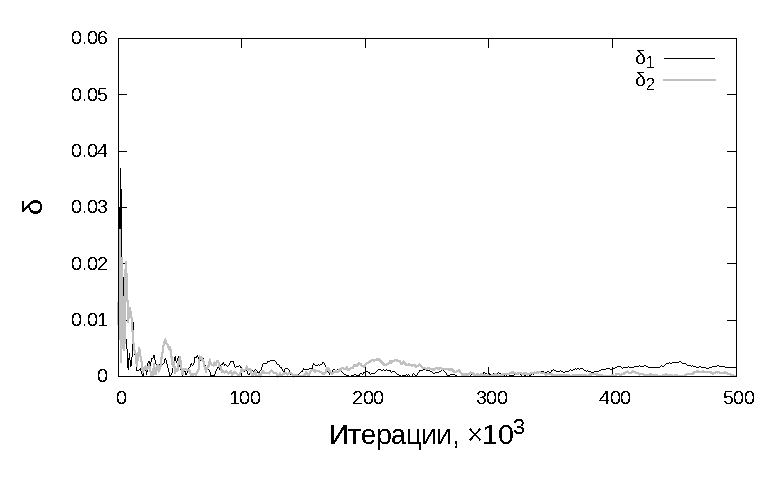
\includegraphics[width=\textwidth]{figs/classic/linear_log_10x_3_samples_10_variance_10_norm.log_0_500.eps}
    \caption{$N \in [0;~5 \cdot 10^5]$}
    \label{fig:classic_var10_n10_begin}
  \end{subfigure}
  \begin{subfigure}[b]{0.3\textwidth}
    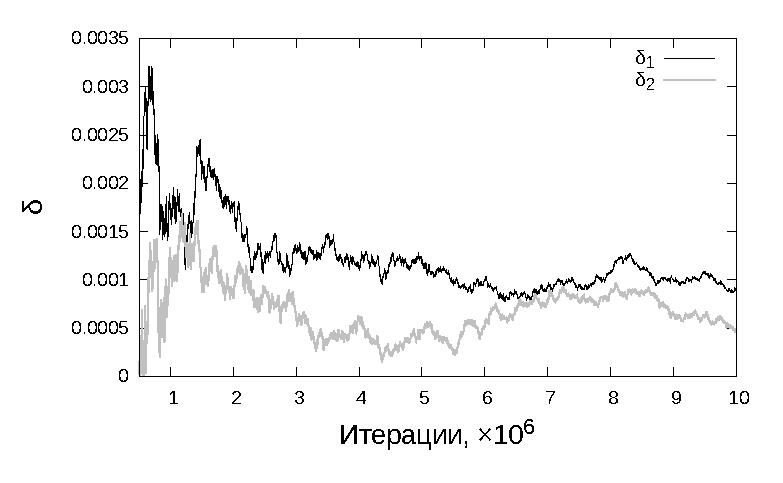
\includegraphics[width=\textwidth]{figs/classic/linear_log_10x_3_samples_10_variance_10_norm.log_500_10000.eps}
    \caption{$N \in [5 \cdot 10^5;~10^7]$}
    \label{fig:classic_var10_n10_middle}
  \end{subfigure}
  \begin{subfigure}[b]{0.3\textwidth}
    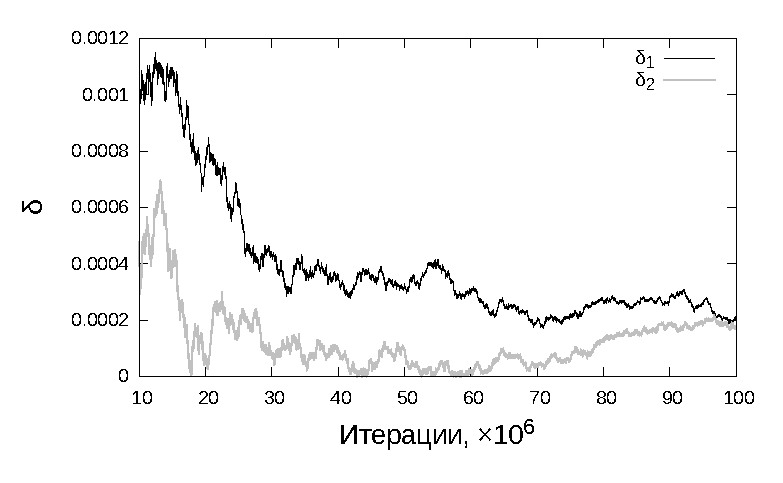
\includegraphics[width=\textwidth]{figs/classic/linear_log_10x_3_samples_10_variance_10_norm.log_end.eps}
    \caption{$N \in [10^7;~10^8]$}
    \label{fig:classic_var10_n10_end}
  \end{subfigure}
  \caption{Зависимость $\delta$ от числа итераций $N$ при $D(\xi) = 10$ и $\ell = 10$.}
  \label{fig:classic_var10_n10}
\end{figure}

\begin{figure}[h!]
  \begin{subfigure}[b]{0.3\textwidth}
    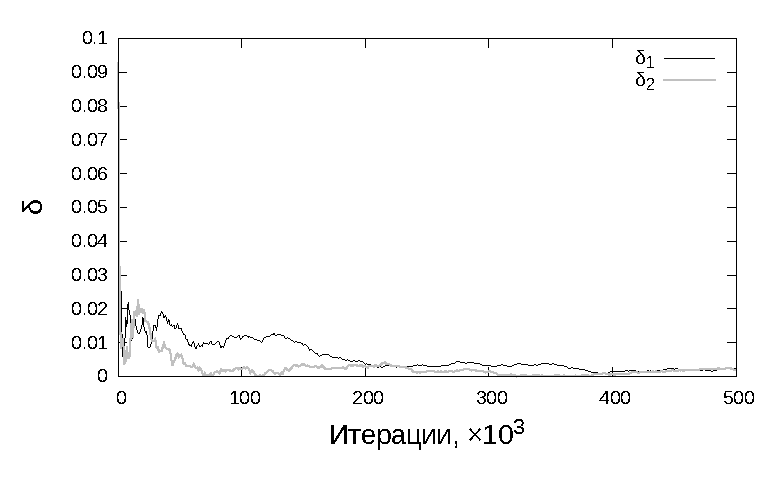
\includegraphics[width=\textwidth]{figs/classic/linear_log_10x_3_samples_10_variance_1_norm.log_0_500.eps}
    \caption{$N \in [0;~5 \cdot 10^5]$}
    \label{fig:classic_var1_n10_begin}
  \end{subfigure}
  \begin{subfigure}[b]{0.3\textwidth}
    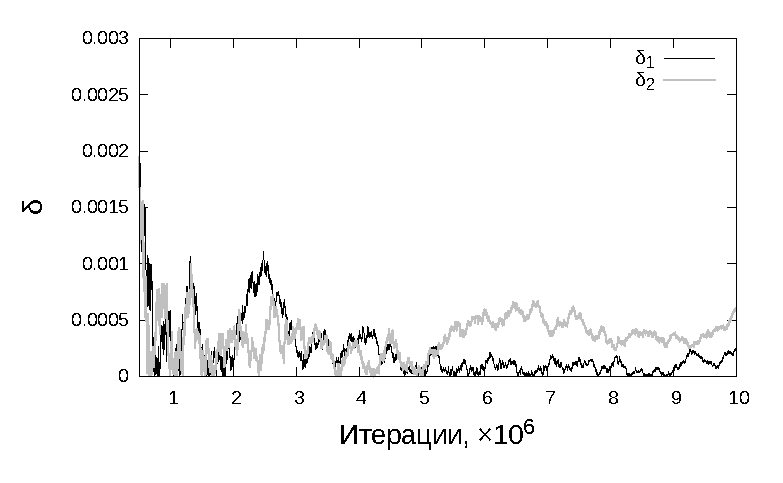
\includegraphics[width=\textwidth]{figs/classic/linear_log_10x_3_samples_10_variance_1_norm.log_500_10000.eps}
    \caption{$N \in [5 \cdot 10^5;~10^7]$}
    \label{fig:classic_var1_n10_middle}
  \end{subfigure}
  \begin{subfigure}[b]{0.3\textwidth}
    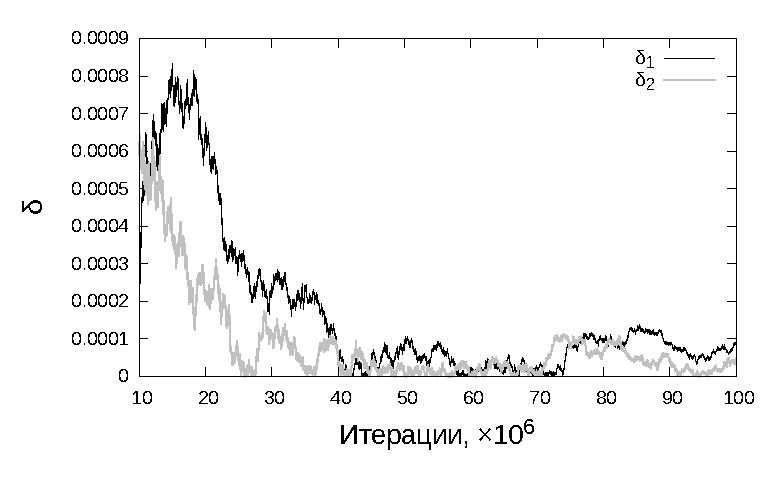
\includegraphics[width=\textwidth]{figs/classic/linear_log_10x_3_samples_10_variance_1_norm.log_end.eps}
    \caption{$N \in [10^7;~10^8]$}
    \label{fig:classic_var1_n10_end}
  \end{subfigure}
  \caption{Зависимость $\delta$ от числа итераций $N$ при $D(\xi) = 1$ и $\ell = 10$.}
  \label{fig:classic_var1_n10}
\end{figure}

\begin{figure}[h!]
  \begin{subfigure}[b]{0.3\textwidth}
    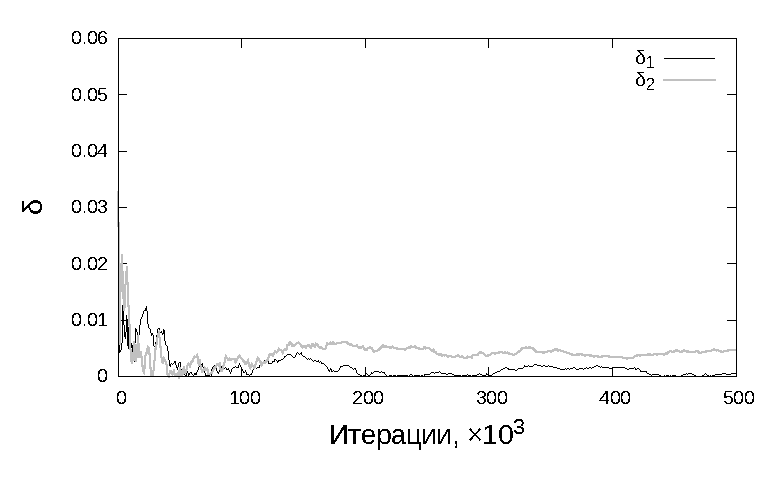
\includegraphics[width=\textwidth]{figs/classic/linear_log_10x_3_samples_50_variance_1_norm.log_0_500.eps}
    \caption{$N \in [0;~5 \cdot 10^5]$}
    \label{fig:classic_var1_n50_begin}
  \end{subfigure}
  \begin{subfigure}[b]{0.3\textwidth}
    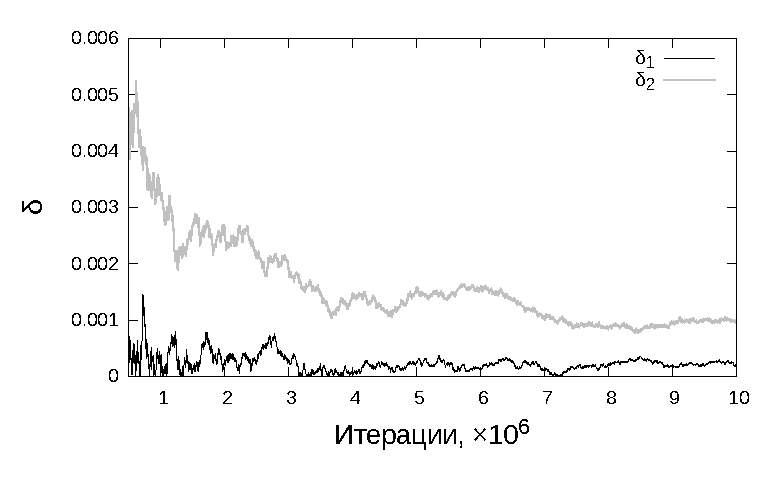
\includegraphics[width=\textwidth]{figs/classic/linear_log_10x_3_samples_50_variance_1_norm.log_500_10000.eps}
    \caption{$N \in [5 \cdot 10^5;~10^7]$}
    \label{fig:classic_var1_n50_middle}
  \end{subfigure}
  \begin{subfigure}[b]{0.3\textwidth}
    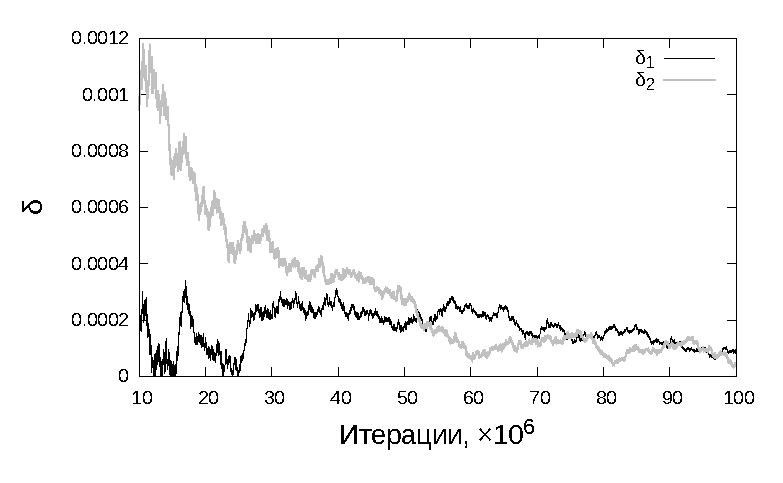
\includegraphics[width=\textwidth]{figs/classic/linear_log_10x_3_samples_50_variance_1_norm.log_end.eps}
    \caption{$N \in [10^7;~10^8]$}
    \label{fig:classic_var1_n50_end}
  \end{subfigure}
  \caption{Зависимость $\delta$ от числа итераций $N$ при $D(\xi) = 1$ и $\ell = 50$.}
  \label{fig:classic_var1_n50}
\end{figure}

На рис. \ref{fig:classic_var10_n10}-\ref{fig:classic_var1_n50}
по оси абсцисс указано количество реализаций $N$, а по
оси ординат для каждого из коэффициентов $a$, $b$ отношение
$\delta = \frac{\sigma_{c.e.} - \sigma_t}{\sigma_t}$, где $\sigma_{c.e.}$~---
значение дисперсии, полученное в вычислительном эксперименте, а
$\sigma_{t}$~--- точное теоретическое значение дисперсии согласно 
\eqref{eq:classic_da}-\eqref{eq:classic_db}.

Как видно, для $N \approx 2.5 \cdot 10^7$ относительное различие
$\frac{\sigma_{c.e.} - \sigma_t}{\sigma_t}$ не
превышает $0.05 \%$ вне зависимости от количества точек, в которых
определена независимая переменная, и значения дисперсии случайной величины.
Это, на наш взгляд, является хорошим результатом и
свидетельствует в пользу корректности обсуждаемого подхода и основной
гипотезы.

\section{Погрешность регрессионных коэффициентов зависимости $n(\lambda)$}

В эксперименте при 17 значениях длины волны был измерен
показатель преломления прозрачного (в исследуемом спектральном
диапазоне) полимера, результаты представлены в таблице \ref{tabl:source_data}.

\begin{table}[h]
  \footnotesize
  \begin{tabular}{| l | r | r | r | r | r | r | r | r | r |} \hline
	$\lambda$, нм	& 435.8		& 447.1		& 471.3		& 486.1		& 501.6		& 546.1		& 577.0		& 587.6		& 589.3		\\ \hline
	$n$				& 1.35715	& 1.35625	& 1.35449	& 1.35349	& 1.35275	& 1.35083	& 1.34968	& 1.34946	& 1.34938	\\ \hline
  \end{tabular}
  \begin{tabular}{| l | r | r | r | r | r | r | r | r |} \hline
	$\lambda$, нм	& 656.3		& 667.8		& 706.5		& 750		& 800		& 850		& 900		& 950			\\ \hline
	$n$				& 1.34768	& 1.34740	& 1.34664	& 1.34607	& 1.34544	& 1.34487	& 1.34437	& 1.34407		\\ \hline
  \end{tabular}
  \caption{Экспериментальные значения коэффициентов преломления.}
  \label{tabl:source_data}
\end{table}

Абсолютная погрешность измерения показателя преломления $\sigma_n$
составляет обычно $(3 \div 10) \cdot 10^{-5}$ во всем диапазоне длин волн, относительная
погрешность определения длины волны $\frac{\sigma_{\lambda}}{\lambda}$ для используемых
дифракционных приборов составляет $(3 \div 30) \cdot 10^{-4}$.

Для предложенной экспертом модели зависимости $n(\lambda)$ требуется
определить погрешность коэффициентов регрессии,
обусловленную экспериментальными погрешностями измерения длины волны
и показателя преломления.

Кроме того, целесообразно найти зависимость
погрешности коэффициентов регрессии от точности эксперимента, что имеет
не только теоретический, но и практический интерес. Например, улучшение
точности измерения показателя преломления $n$ до $2 \cdot 10^{-5}$ требует значительных
усилий (и затрат), но если при этом погрешность определения коэффициентов
регрессионной модели практически не изменится, то соответствующая работа по
модернизации экспериментальной установки не имеет смысла. Точно так же,
при улучшении точности определения показателя преломления имеет не
только теоретический, но и практический смысл вопрос о том, насколько требуется
улучшить точность определения длины волны, чтобы
обеспечить значительное снижение погрешности определения коэффициентов
регрессии.

Экспертом была предложена функциональная зависимость
следующего вида:
\begin{equation}
  n(\lambda) = a + \frac{b}{\lambda^2} + \frac{c}{\lambda^4}.
  \label{eq:polymer_formula}
\end{equation}

Для указанного вида нелинейной регрессии с помощью АЛМ были
определены оптимальные коэффициенты регрессии, обеспечивающие
среднеквадратичную ошибку $\approx 3.97 \cdot 10^{-9}: a = 1.33344; b = 2841.63; c = 1599.27;$
длина волны измеряется в нанометрах.

Вычисление погрешностей коэффициентов регрессионной модели было
проведено для ряда комбинаций погрешностей определения длины волны (в
относительных единицах) и показателя преломления (также в относительных
единицах), в каждом случае проводилась статистическая обработка миллиона
реализаций. Некоторые результаты вычислительного эксперимента приведены
в таблицах \ref{tabl:inacc_a}-\ref{tabl:inacc_c}.

\begin{table}[h]
  \center
  \begin{tabular}{| l | c | c | c |} \hline
	\backslashbox{$\frac{\sigma_{\lambda}}{\lambda}$}{$\frac{\sigma_n}{n}$}				& $2 \cdot 10^{-5}$		& $1 \cdot 10^{-4}$		& $3 \cdot 10^{-4}$		\\ \hline
	$10^{-3}$		& $1.255 \cdot 10^{-2}$	& $5.54 \cdot 10^{-2}$	& $1.656 \cdot 10^{-1}$	\\ \hline
	$10^{-2}$		& $6.32 \cdot 10^{-2}$ 	& $8.24 \cdot 10^{-2}$	& $1.753 \cdot 10^{-1}$	\\ \hline
  \end{tabular}
  \caption{Относительная погрешность определения коэффициента регрессии $a$.}
  \label{tabl:inacc_a}
\end{table}
\begin{table}[h]
  \center
  \begin{tabular}{| l | c | c | c |} \hline
	\backslashbox{$\frac{\sigma_{\lambda}}{\lambda}$}{$\frac{\sigma_n}{n}$}				& $2 \cdot 10^{-5}$		& $1 \cdot 10^{-4}$		& $3 \cdot 10^{-4}$		\\ \hline
	$10^{-3}$		& $2.14$				& $8.68$				& $25.4$				\\ \hline
	$10^{-2}$		& $13.6$				& $15.9$				& $28.5$				\\ \hline
  \end{tabular}
  \caption{Относительная погрешность определения коэффициента регрессии $b$.}
  \label{tabl:inacc_b}
\end{table}
\begin{table}[h]
  \center
  \begin{tabular}{| l | c | c | c |} \hline
	\backslashbox{$\frac{\sigma_{\lambda}}{\lambda}$}{$\frac{\sigma_n}{n}$}				& $2 \cdot 10^{-5}$		& $1 \cdot 10^{-4}$		& $3 \cdot 10^{-4}$		\\ \hline
    $10^{-3}$		& $1.15 \cdot 10^3$		& $1.426 \cdot 10^3$	& $1.454 \cdot 10^3$	\\ \hline
	$10^{-2}$		& $1.45 \cdot 10^3$		& $1.456 \cdot 10^3$	& $1.47 \cdot 10^3$		\\ \hline
  \end{tabular}
  \caption{Относительная погрешность определения коэффициента регрессии $c$.}
  \label{tabl:inacc_c}
\end{table}

Для $\frac{\sigma_{\lambda}}{\lambda} < 10^{-4}$ погрешности первого и второго коэффициентов
регрессии очень слабо зависят от дальнейшего увеличения точности
определения длины волны и почти линейно зависят от точности измерения
показателя преломления. Для $\frac{\sigma_n}{n} \approx 2 \cdot 10^{-5}$
и $\frac{\sigma_{\lambda}}{\lambda} \approx 5 \cdot 10^{-4}$ относительная
погрешность определения составляет $\approx 7 \cdot 10^{-3}$ для первого коэффициента
регрессии и $\approx 7 \cdot 10^{-4}$ для второго (интересно отметить, что второй
коэффициент регрессии определяется точнее). Погрешность определения
третьего коэффициента регрессии высока, что, очевидно, связано с
незначительным вкладом третьего слагаемого в \eqref{eq:polymer_formula} в показатель преломления:
изменение этого слагаемого слабо влияет на общую величину
среднеквадратичного отклонения, следовательно, этот компонент определяется с низкой точностью.

\section{Заключение}

\begin{enumerate}
  \item Предложенный в настоящей работе метод определения погрешностей коэффициентов
    регрессии может использоваться при любом распределении
    вероятности ошибки зависимых и независимых переменных регрессии,
    включая различные виды распределения ошибки для разных переменных, а
    также для одной переменной в различных экспериментальных точках.
  \item Предложенный метод будет давать несколько разные значения погрешностей при
    использовании различных функционалов ошибки $S$. Такая ситуация
    не является необычной и, например, коэффициенты регрессии будут разными,
    если по стандартному методу наименьших квадратов (МНК) минимизируется
    сумма квадратов расстояний по оси, соответствующей зависимой переменной, от экспериментальных точек до
	аппроксимирующей регрессионной модели согласно \eqref{eq:S} или же минимизируется сумма
    евклидовых расстояний от экспериментальных точек до аппроксимирующей
	модели аналогично известной работе Пирсона \cite{pearson1901}.

	С нашей точки зрения, выбор оптимального функционала G
	проводится экспертом, исходя, прежде всего, из анализа погрешностей
	определения зависимых и независимых переменных. В самом деле, если
	независимая переменная определяется точно, то МНК предпочтителен, а при
	близких погрешностях переменных подход Пирсона представляется
	предпочтительным.
  \item Для оптимизации коэффициентов регрессии использовался
	АЛМ в стандартной форме, когда минимизируется функционал типа \eqref{eq:S}. Как
	указано выше, этот вариант МНК корректен, когда погрешность независимой
	переменной мала, а в общем случае метод АЛМ следует модифицировать,
	минимизируя суммы вида $(\frac{\Delta x_i}{\sigma_{x_i}})^2 + (\frac{\Delta y_i}{\sigma_{y_i}})^2$. Однако для конкретных
	вычислительных экспериментов, результаты которых представлены в
	настоящей работе, возможно использование АЛМ в стандартной форме.

	В самом деле, заранее предполагается, что независимая
	переменная известна точно: $\forall i : D(x_i) = 0$. Далее, можно показать, что
	использование функционала \eqref{eq:S} в вычислительном эксперименте
	корректно, если $\frac{\sigma_n}{\sigma_{\lambda}} > \frac{dn}{d\lambda}$ и для анализируемого полимера это
	условие выполняется с кратным запасом.
\end{enumerate}

Таким образом, в настоящей работе предложен метод определения
погрешностей коэффициентов регрессионной модели, включая случай нелинейной регрессии. В
вычислительном эксперименте получено хорошее соответствие теоретически описанному случаю, когда
стандартное отклонение коэффициентов регрессии определяется точно.
Показана целесообразность применения предложенного вычислительного
алгоритма при анализе конкретных физических экспериментов.

\FloatBarrier

\bibliographystyle{babunsrt-lf}
%\bibliographystyle{babunsrt}
%\bibliographystyle{unsrt}
\bibliography{bibliography}

\end{document}
